% ---------------------------------------------------------------------------
% Client-assisted homomorphic inference for a genomic foundation model
%
% Build:  latexmk -pdf main.tex
% Figures: paper-docs/scripts/figures.py  (writes ../figures/*.pdf)
% Lint:    paper-docs/scripts/check_numbers.py
%
% Every number in this document must exist in paper-docs/evidence/*.yaml.
% Read paper-docs/AGENTS.md and paper-docs/context/00_terminology.md before editing.
% ---------------------------------------------------------------------------

\documentclass{IEEEtran}

% ---------------------------------------------------------------------------
% House preamble.
%
% Base: the single-column layout used for the group's previous submission, kept
% deliberately identical so the two papers read as a series.
% Additions over that base: cmap + glyphtounicode (correct PDF text extraction and
% copy-paste), full hyperref PDF metadata, and numbered invariant/proposition
% environments for the threat model.
% ---------------------------------------------------------------------------

% Latin Modern gives proper T1 outlines rather than the bitmap CM defaults.
\usepackage{lmodern}
\usepackage[T1]{fontenc}
% Neither CM nor Latin Modern ships bold small-caps, so the \bfseries\scshape section
% headings below have always silently rendered as bold upright. Declaring that
% substitution explicitly changes nothing on the page and stops the warning. If real
% bold small-caps headings are wanted, that needs a different text font, which would
% change the house look this preamble deliberately shares with the previous submission.
\DeclareFontShape{T1}{lmr}{bx}{sc}{<->ssub*lmr/bx/n}{}
\usepackage[utf8]{inputenc}
\usepackage{cmap}
\ifdefined\pdfgentounicode \input{glyphtounicode} \pdfgentounicode=1 \fi

\usepackage[a4paper, top=2.0cm, bottom=2.4cm, left=1.5cm, right=1.5cm, columnsep=0.65cm]{geometry}

\usepackage{amsmath}
\usepackage{amssymb}
\usepackage{amsthm}
\usepackage{booktabs}
\usepackage{multirow}
\usepackage{array}
\usepackage{tabularx}
\usepackage{graphicx}
\usepackage{xcolor}
\usepackage{microtype}
\usepackage{url}
\usepackage{titlesec}
\usepackage{caption}
\usepackage{enumitem}
\usepackage{fancyhdr}
\usepackage{natbib}
\usepackage{algorithm}
\usepackage{algpseudocode}
\usepackage{hyperref}

% algpseudocode defines \Call using \ifthenelse{\equal{#2}{}} to detect an empty
% argument list. \equal expands its arguments, so any \Call whose arguments contain
% a macro -- a nested \Call, as in Algorithms 1 and 2 -- makes the test blow up with
% "Argument of \equal has an extra }". \@ifmtarg performs the same emptiness test
% without expanding, so the redefinition below is behaviourally identical for the
% empty case and simply correct for the non-empty one.
\usepackage{ifmtarg}
\makeatletter
\renewcommand{\Call}[2]{\textproc{#1}\@ifmtarg{#2}{}{(#2)}}
\makeatother

% Line numbers belong to the reviewer-facing build only, so referees can cite a
% page and line. The default build is the clean preprint: scripts/build.sh
% regenerates buildmode.tex on every run, writing \reviewbuildtrue only when
% called with --review. The \reviewbuildfalse below is the fallback for a direct
% latexmk or tectonic invocation that bypasses the script.
\usepackage[switch]{lineno}
\newif\ifreviewbuild
\reviewbuildfalse
\InputIfFileExists{buildmode.tex}{}{}

\bibliographystyle{abbrvnat}

% --- Sectioning -------------------------------------------------------------
\titleformat{\section}{\normalfont\large\bfseries\scshape}{\thesection}{1em}{}
\titleformat{\subsection}{\normalfont\normalsize\bfseries}{\thesubsection}{1em}{}

% --- Lists, captions, spacing ----------------------------------------------
\setlist[itemize]{leftmargin=*, topsep=2pt, itemsep=1pt}
\setlist[enumerate]{leftmargin=*, topsep=2pt, itemsep=1pt}
\captionsetup{font=small, labelfont=bf}
\raggedbottom
\setlength{\emergencystretch}{2em}
\setlength{\parindent}{0pt}
\setlength{\parskip}{4pt plus 1pt minus 1pt}
\hbadness=10000 \vbadness=10000 \hfuzz=4pt \vfuzz=4pt

% --- Tables -----------------------------------------------------------------
\newcolumntype{Y}{>{\raggedright\arraybackslash}X}
\newcolumntype{R}{>{\raggedleft\arraybackslash}X}

% --- Float placement --------------------------------------------------------
% Every figure is authored at the full 18cm text width and every wide table spans
% both columns, so this document leans heavily on double-column floats. The LaTeX
% defaults are tuned for occasional single-column floats and will strand one
% full-width float on an otherwise blank page rather than let it share with text.
% These limits let a page carry several floats plus body text.
\setcounter{topnumber}{3}
\setcounter{bottomnumber}{2}
\setcounter{totalnumber}{4}
\setcounter{dbltopnumber}{3}
\renewcommand{\topfraction}{0.92}
\renewcommand{\bottomfraction}{0.6}
\renewcommand{\textfraction}{0.07}
\renewcommand{\floatpagefraction}{0.8}
\renewcommand{\dbltopfraction}{0.92}
% Only surrender a whole page to double-column floats when they genuinely fill
% it; otherwise LaTeX strands one figure on a mostly blank page.
\renewcommand{\dblfloatpagefraction}{0.9}
\setlength{\dbltextfloatsep}{12pt plus 2pt minus 2pt}
% Standard LaTeX defers a double-column float to the next page and cannot place
% one at the bottom, which is what produces the stranded pages. dblfloatfix
% restores bottom placement and keeps floats in declaration order.
\usepackage{dblfloatfix}
% This document declares 19 floats, many of them double-column. Once LaTeX runs
% out of float storage it force-flushes the queue to float pages and ignores the
% fractions above, which is what strands a half-full figure on its own page.
\extrafloats{64}

% --- Page furniture ---------------------------------------------------------
\pagestyle{fancy}\fancyhf{}\fancyfoot[R]{\small\thepage}
\renewcommand{\headrulewidth}{0pt}\renewcommand{\footrulewidth}{0.4pt}

% --- Theorem-like environments for the threat model -------------------------
\newtheorem{invariant}{Invariant}
\newtheorem{proposition}{Proposition}

% --- Links ------------------------------------------------------------------
\hypersetup{
  colorlinks=true,
  linkcolor=blue!60!black,
  citecolor=blue!60!black,
  urlcolor=blue!60!black,
  pdftitle={Client-assisted homomorphic inference for a genomic foundation model},
  pdfauthor={Christos Galanopoulos; Kimon Antonios Provatas; Ilias Georgakopoulos-Soares},
  pdfsubject={Privacy-preserving inference; CKKS homomorphic encryption; genomic language models},
  pdfkeywords={homomorphic encryption; CKKS; genomic privacy; transformer inference; GPU}
}
\pdfstringdefDisableCommands{\def\texttt#1{#1}}

% --- Evidence tags ----------------------------------------------------------
% Used only in internal drafts to mark measurement status while writing. The
% submission builder removes them; they must not survive into the final PDF.
\newcommand{\Vtag}{\textcolor{green!45!black}{\footnotesize[V]}}
\newcommand{\Utag}{\textcolor{red!60!black}{\footnotesize[U]}}
\newcommand{\Atag}{\textcolor{orange!70!black}{\footnotesize[A]}}

% --- Figure placeholder -----------------------------------------------------
% Author sections against these, then swap for \includegraphics once the figure
% script has produced the PDF.
\newcommand{\figplaceholder}[2]{%
  \begin{center}\fbox{\begin{minipage}{0.92\textwidth}\centering\vspace{1.2cm}
  \textbf{[figure: #1]}\\[4pt]\small #2\vspace{1.2cm}\end{minipage}}\end{center}}


\graphicspath{{../figures/}{figures/}}

\begin{document}

% ---------------------------------------------------------------------------
% Front matter: title, authors, graphical abstract, abstract, key points.
%
% Framing follows the project objective in CLAUDE.md: this is a FEASIBILITY STUDY.
% The question is whether DNAGPT inference can run under homomorphic encryption, and where
% correctness, performance, or memory would stop a complete encrypted deployment.
% Feasibility and practicality are reported as SEPARATE verdicts. A correct-but-slow encrypted
% path is a valid, publishable outcome; nothing is tuned to force "practical".
%
% Source: context/01_scenario_and_motivation.md, context/05_claims_and_qualifiers.md
% ---------------------------------------------------------------------------

\title{\vspace{-1.2cm}\textbf{Feasibility of Homomorphic Inference for a Genomic Foundation
Model: A Client-Assisted CKKS Evaluation of DNAGPT}\vspace{-0.2cm}}

\author{%
  \begin{minipage}{0.96\textwidth}
  \raggedright
  \textbf{Christos Galanopoulos$^{1,*}$, Kimon Antonios Provatas$^{1}$,
  Ilias Georgakopoulos-Soares$^{1,*}$}\\[2pt]
  \normalsize $^{1}$The University of Texas at Austin, Austin, TX, USA\\[2pt]
  \small $^{*}$Corresponding authors: \texttt{TODO@utexas.edu}\\[2pt]
  \small\textit{Homomorphic encryption $\cdot$ Genomic privacy $\cdot$ Transformer inference
  $\cdot$ GPU acceleration}
  \end{minipage}
}
\date{}

\maketitle
\thispagestyle{fancy}

% The graphical abstract is temporarily excluded pending evidence-safe regeneration; see
% paper-docs/TODO.md. The generated asset contains timing and client-memory claims whose
% supporting logs are not present in the repository.

% --- Abstract ---------------------------------------------------------------
\section*{Abstract}

\textbf{Motivation.} Human genomic sequence is identifying, cannot be replaced after disclosure,
and is precisely the input that genomic foundation models are designed to interpret. We ask
whether a provider can execute a released genomic transformer without receiving genomic values in
plaintext, and whether correctness, memory, or cost prevents a complete encrypted deployment.

\textbf{Results.} We validate DNAGPT on genomic-signal recognition, promoter and splice-site
classification, and mRNA abundance regression, then freeze an independently checked numerical
reference. We evaluate two CKKS designs. In the evaluated pure non-interactive configuration,
polynomial nonlinearities permit a released-weight block to complete, but context and evaluation
keys exceed the tested $80$~GB memory envelope when configured for composition. In the
client-assisted design, the provider evaluates linear operations on ciphertexts while the
key-holding data owner evaluates exact LayerNorm, causal softmax, and GELU at fixed boundaries.
The resulting released-weight block at the task-defined prompt matches its validated plaintext
reference with $4.64\times10^{-9}$ relative error against a $4\times10^{-2}$ tolerance fixed in
advance, while the evaluating process peaks at $9.6$~GiB of GPU memory.

\textbf{Conclusions.} Correctness is not the barrier. The protocol moves the accelerator-memory
barrier by replacing deep non-interactive segments with fresh encryption at declared boundaries;
bounded caching separately prevents encoded plaintexts from accumulating in host memory. The
systems campaign removes repeated host encoding while preserving an asserted operation schedule,
packing, depth, and reference. Client-assisted DNAGPT evaluation is feasible at the demonstrated
scope. Its practicality remains unresolved until the retained implementation is timed on a clean,
dedicated node.

\textbf{Availability.} Code, evaluation harnesses, and the evidence record are maintained at
\url{https://github.com/Georgakopoulos-Soares-lab/private_genomic_dnagpt}.

% --- Key points -------------------------------------------------------------
\section*{Key Points}

\begin{itemize}
  \item We test whether a released genomic foundation model can be evaluated under homomorphic
        encryption, and report feasibility and practicality as separate verdicts rather than as
        one.
  \item The model is validated first on three genomic task families; the independent numerical
        reference is itself asserted against every upstream block before it is used to verify
        encrypted execution.
  \item Correctness is not a barrier: a complete transformer block at the task's own prompt length
        matches the validated plaintext reference to $4.64\times10^{-9}$ relative error, seven
        orders of magnitude inside the tolerance fixed before the run.
  \item Memory is a barrier that design moves. Approximating the nonlinearities under encryption
        exceeded the tested $80$~GB accelerator envelope at composition; client assistance yields
        a $9.6$~GiB evaluating-process GPU peak for the retained block.
  \item Bounded caching addresses a distinct host-memory problem. Runtime assertions confirm that
        the complete operation schedule, packing, depth, and reference remain unchanged while
        repeated plaintext encoding is removed.
  \item The data owner requires no GPU. Practicality remains a separate, unresolved verdict until
        the retained implementation has a clean dedicated-node timing measurement.
\end{itemize}


% ---------------------------------------------------------------------------
% 1 Introduction
% Source: context/01_scenario_and_motivation.md, context/02_research_timeline.md
%
% This paper asks a feasibility question and answers it. The shape of the section is therefore:
% tension -> the question -> why the question is hard -> how we answer it -> the two verdicts.
% ---------------------------------------------------------------------------

\section{Introduction}

Human genomic sequence carries an unusually persistent confidentiality risk. It can identify its
contributor and, through familial relationships, reveal information about people who never supplied
a sample; re-identification has been demonstrated even when conventional identifiers were
removed~\cite{gymrek2013,erlich2018}. A disclosed genome also cannot be replaced in the manner of a
password or access token. European data-protection law accordingly treats genetic data as a special
category~\cite{gdpr}. The same sequence is the input on which genomic foundation models derive
their value: DNAGPT serves classification, regression, and generation tasks through a common
transformer backbone~\cite{dnagpt2023}. When that model is served rather than distributed, a data
owner without accelerator hardware must otherwise disclose the sequence to the provider or forgo
the inference. Nor is handing over an embedding a way out: per-token embeddings from DNA foundation
models have been shown to permit near-perfect reconstruction of the underlying
sequence~\cite{dnaembeddinginversion2026}. Homomorphic encryption offers a route for the provider to
compute without receiving the genomic values in plaintext.

DNAGPT's public release makes the experiment auditable and also makes this particular artifact
available for local execution. We use it as a reproducible surrogate for a genomic model offered
only as a service by policy or contract. Under that premise, client-assisted evaluation gives a
CPU-equipped data owner access to the served model without disclosing the genome.

Against this deployment premise, we ask: can inference with a released genomic foundation model be
executed under homomorphic encryption, and where would correctness, performance, or memory prevent
a complete encrypted deployment? The question contains two verdicts that should not be collapsed.
Feasibility asks whether the released computation can be executed faithfully within the available
cryptographic and memory budget. Practicality asks whether its resource cost supports a target use.
A correct but slow encrypted path is therefore evidence: it resolves the first question while
locating the work needed to change the second.

The technical difficulty is concentrated where a transformer departs from affine arithmetic. CKKS
supports approximate packed arithmetic and maps naturally to dense projections, rotations, and
accumulations~\cite{ckks2017}; LayerNorm, softmax, and GELU are not native CKKS operations. A
non-interactive evaluator must approximate them with polynomial circuits, lengthening the
multiplicative path and increasing the context, bootstrapping, and evaluation-key material that
must be resident. Moving the exact functions to the key holder shortens those paths and resets the
depth budget, but introduces interaction and a different threat model. Earlier systems establish
both directions: THOR demonstrates non-interactive homomorphic transformer inference; THE-X and
Safhire use interactive workflows in which the client evaluates nonlinear
functions~\cite{thor,thex2022,safhire2025}. The division of labor is therefore established prior
art. What has not been reported is an auditable account of the numerical behavior, memory,
interaction, and executed work that results when it is applied end to end to a released genomic
transformer, at that model's own task prompt, with its weights and nonlinear formulas unmodified.

That choice buys exactness and depth. Evaluating LayerNorm, softmax, and GELU at the key holder
keeps the released formulas intact, so no polynomial approximation of a nonlinearity enters the
model, and it bounds multiplicative depth by the longest encrypted segment rather than by network
depth. The price is an online key holder and a protocol that is not the fastest available:
non-interactive systems report lower cost for transformer inference, and Section~\ref{sec:related}
treats those figures as cross-paper context rather than as a controlled benchmark.

We begin by establishing that the target computation is meaningful and independently reproducible.
The released DNAGPT paths are evaluated across genomic-signal recognition, promoter and splice-site
classification, and mRNA abundance regression, with task outputs frozen before encrypted work.
The validation records the released float32 path, checks an independent NumPy float64 lineage
against a float64-cast PyTorch shadow at $2\times10^{-5}$ for every released block and the task
head, and then compares encrypted execution with the NumPy reference. We build two CKKS designs: a
non-interactive circuit with polynomial nonlinearities, and a client-assisted circuit whose fixed,
non-adaptive boundaries evaluate the released nonlinearities exactly. Instrumented evaluations
record where each design stops in correctness and memory, while runtime assertions preserve the
complete cryptographic operation schedule throughout the systems campaign.

The results separate three candidate barriers and resolve two of them. Correctness holds: the
client-assisted design evaluates all twelve released blocks and the task head at the $103$-token
prompt, and for the one input evaluated it reproduces the frozen plaintext label with
$8.56\times10^{-9}$ relative margin error against a $4\times10^{-2}$ tolerance fixed before
evaluation. Accelerator memory holds as well, and for a structural reason: because multiplicative
depth is bounded by the longest segment between client boundaries instead of by network depth, it
stays at $13$ for the complete model, device-wide GPU memory used reaches $9839$~MiB without growth
across the twelve blocks, and no homomorphic bootstrap is required at any point. Bounded caching
separately prevents encoded plaintexts from accumulating across host-side stages. The evaluated
non-interactive design, by contrast, completes one released-weight block but exceeds the tested
$80$~GB envelope while loading its composition context and evaluation keys, placing that barrier in
the nonlinear schedule rather than in the model's dense maps. Cost is the barrier that remains: one
encrypted classification takes $1.86$~hours on an A100 GPU node, which forecloses interactive use
in the evaluated form, and sampled GPU utilization peaks at $51\%$, locating headroom without
attributing it. These memory and timing figures are specific to the evaluated backend, packing, and
parameters.

The paper makes the following contributions:

\begin{itemize}
  \item \textbf{Complete-model feasibility.} All twelve released DNAGPT blocks and the task head
        execute at the $103$-token task prompt from encrypted embedded vectors, with unmodified
        released weights and nonlinear formulas and without homomorphic bootstrap; the one
        evaluated prompt reproduces the reference label. To our knowledge this is the first
        complete forward pass of a released, pretrained genomic foundation model evaluated under
        CKKS; prior homomorphic transformer evaluations over biological sequence data have targeted
        small, purpose-trained classifiers~\cite{idash24descriptor,encrypteddashformer}.
  \item \textbf{Model-faithful, reproducible evaluation.} The protocol, packing, checked operation
        schedule, predeclared tolerance, and three-link float32--float64--encrypted validation
        chain make the complete execution independently inspectable.
  \item \textbf{Measured systems anatomy and scoped negative results.} We report complete-model
        cost, interaction, depth, and memory; the stage-bounded cache that makes host-side reuse
        executable; and the memory boundary reached by the evaluated non-interactive configuration.
\end{itemize}

\begin{figure*}[!t]\centering
  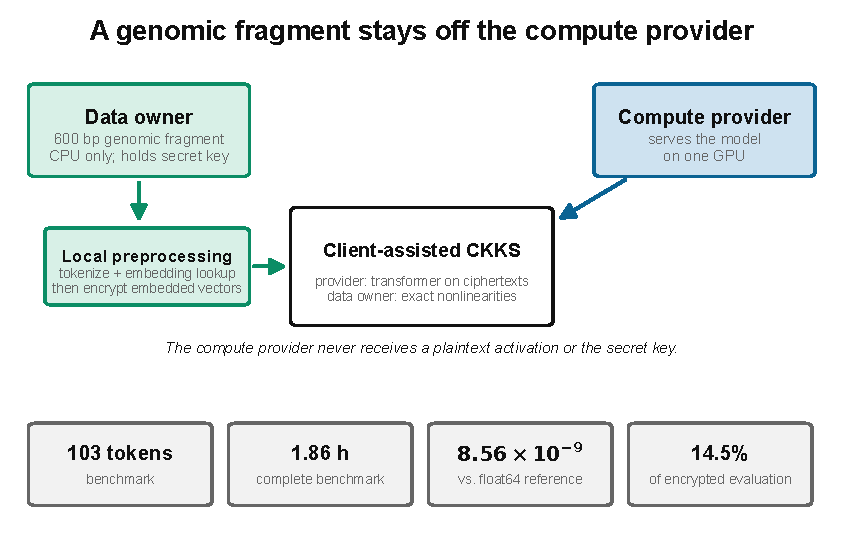
\includegraphics[width=\textwidth]{fig_graphical_abstract.pdf}
  \caption{Study overview and measured complete-classifier result. The data owner retains the
  secret key and evaluates exact nonlinearities; the compute provider evaluates encrypted linear
  algebra. The reported execution begins at encrypted embedded vectors and covers one genomic-signal input.}
  \label{fig:overview}
\end{figure*}

% ---------------------------------------------------------------------------
% 2 Background
% Source: docs/shared/backend_selection.md, docs/overview.md,
%         docs/hybrid/t123_walkthrough.md §3 (glossary) and §3.1
% ---------------------------------------------------------------------------

\section{Background}

\subsection{DNAGPT and the genomic task families}
DNAGPT is an autoregressive transformer adapted to sequence and numerical tasks over
DNA~\cite{dnagpt2023}. We evaluate its released $0.1$-billion-parameter configuration. The backbone has
$12$ transformer blocks, hidden width $768$, and $12$ causal-attention heads of width $64$. Its
feed-forward sublayer expands to width $3{,}072$. DNA is represented through $6$-mer tokenization
and combined with task-format tokens before entering the transformer.

Each block follows the structure that determines the encrypted circuit: LayerNorm; query, key, and
value projections; causal self-attention; an output projection and residual; a second LayerNorm;
then an expanded MLP with GELU and another residual. The dense maps apply fixed model weights.
LayerNorm and GELU apply nonlinear functions to the activations, while attention introduces products
between two data-dependent quantities and normalizes them with a softmax.

The release includes fine-tuned heads for genomic-signal recognition and mRNA abundance regression,
but none for the genome-understanding benchmark, so Section~\ref{sec:baseline} evaluates that
backbone with a locally fine-tuned linear head. All three task families predate DNAGPT and carry
established task-specific baselines~\cite{deepgsr,xpresso,dnabert2}, against which
Section~\ref{sec:baseline} establishes model fidelity; the encrypted study then uses the
signal-recognition path as its task-length anchor.

\subsection{CKKS}
CKKS supports approximate arithmetic on packed vectors of real or complex
values~\cite{ckks2017}. Encoding places many values into the slots of one plaintext, which is then
encrypted under the data owner's key. Addition and multiplication act slotwise across the packed
vector, while rotations move values between slots. This single-instruction, multiple-data model is
a natural match for transformer activations: a rotation-and-diagonal schedule can express a public
matrix transform as ciphertext--plaintext multiplication and accumulation.

Not every transformer product has a public operand. Query--key scoring multiplies two encrypted
projections of the input, and attention context multiplies encrypted attention weights by encrypted
values. Those operations require ciphertext--ciphertext multiplication and relinearization. The
distinction is about data ownership rather than implementation convenience: public weights and
masks remain plaintext, while every query-derived operand remains encrypted at the server.

CKKS controls approximate fixed-point scale through rescaling. A multiplication consumes a level
from a finite modulus chain, and the computation fails once that multiplicative budget is exhausted.
Bootstrapping can refresh a ciphertext without decryption, while fresh client encryption can reset
the budget in an interactive protocol. Both choices carry system costs, so multiplicative depth is
an architectural resource rather than only a cryptographic parameter.

\subsection{Why the nonlinearities are the architecture}
CKKS directly supplies polynomial arithmetic, but a transformer requires inverse square root in
LayerNorm, exponentiation and normalization in softmax, and GELU. A non-interactive circuit must
replace these functions with polynomial approximations over declared input ranges. Higher-degree
approximations consume additional multiplicative depth; across repeated blocks, the evaluator must
provide a deeper context, a bootstrapping schedule, or both. Larger modulus chains and refresh
operations also increase the context and evaluation-key material that must remain resident.

The alternative is to place exact functions at declared client boundaries, which removes
approximation-range calibration and resets the encrypted depth budget but requires an online client
and exposes intermediate activations to it. The choice between polynomial approximation and client
evaluation therefore determines memory, interaction, depth, and the threat model.
Section~\ref{sec:protocol} evaluates both designs and reports where each stops.

\subsection{Evaluated software backends}
We separate correctness semantics from the performance path. OpenFHE provides CKKS context and
security-parameter construction, encoding, rotations, polynomial evaluation, and approximate
bootstrapping~\cite{openfhe}. It supplies the reference behavior used to validate local encrypted
operators and the non-interactive design. The evaluated GPU backend interoperates with those
representations and provides CUDA implementations of the server-side CKKS operations; all reported
accelerator measurements use that path. Python, NumPy, and PyTorch construct and validate the frozen
plaintext reference, but they do not participate in encrypted performance measurements.

We also evaluated the Boolean/integer-oriented TFHE-rs path and Concrete ML's client/server
workflow~\cite{concreteml,tfhers}; their available GPU acceleration and ciphertext expansion were
less suitable for this matrix-heavy graph than the already validated CKKS path, and a separate CKKS
wrapper lacked the refresh and general nonlinear-function support the non-interactive baseline
needs. These decisions select among the software paths tested here. They do not establish that CKKS
is the only scheme able to express encrypted transformer inference.

% ---------------------------------------------------------------------------
% 9 Related work
% Sources verified in reviews/2026-08-08-paper-sources.md.
% ---------------------------------------------------------------------------

\section{Related work}

\subsection{Private transformer inference}

Private neural-network inference has long combined cryptographic tools according to the
operation being evaluated. Gazelle established an influential hybrid design in which
homomorphic encryption handles linear layers and garbled circuits handle
nonlinearities~\cite{gazelle2018}. Transformer systems inherited this decomposition but had
to contend with attention, normalization, and activation functions at substantially greater
scale. Iron, Nimbus, and BumbleBee combine homomorphic encryption with secret sharing,
oblivious transfer, and specialized two-party protocols for transformer
inference~\cite{iron2022,nimbus2024,bumblebee2025}. Their protocols optimize a joint secure
computation between parties; the present work instead keeps the server's linear path in CKKS
and assigns exact nonlinear evaluation to the data owner at explicit boundaries. This choice
changes both the security contract and the allocation of work between the parties.

Safhire is the closest architectural antecedent~\cite{safhire2025}. It likewise places
homomorphically evaluated linear layers on the server, then has the client decrypt an
intermediate, apply the nonlinearity in plaintext, and return a fresh encryption. Safhire
studies convolutional networks and adds randomized output permutation to make reconstruction
from released intermediates harder. We therefore do not claim the client-assisted pattern as
new. The contribution here is to test that pattern on a released genomic transformer at its
task-defined prompt, retain the released weights and exact nonlinearities, verify the
encrypted block through an independently checked plaintext reference, and expose the resulting
arithmetic, boundary schedule, and memory behavior. This evaluation applies the established
protocol pattern to a released genomic transformer with a reproducible verification chain.

THOR demonstrates full non-interactive transformer evaluation under homomorphic encryption using
a circuit and packing strategy designed for that objective, including diagonal-major organization
and compact packing~\cite{thor}. Its result establishes that the memory wall observed here belongs
to the evaluated backend, parameters, packing, and circuit. Client assistance addresses a distinct
engineering question: whether released computation can be preserved when the data owner is
available to evaluate exact nonlinearities at declared boundaries.

\subsection{Homomorphic encryption for genomics}

Homomorphic encryption already has a substantial genomic-computing lineage. The iDASH secure
genome analysis competition evaluated encrypted association studies, sequence search, and
related privacy-preserving workflows~\cite{idash2018}. Private genomic-query systems combine
homomorphic encryption with hashing and set-intersection techniques to test for variants
without disclosing either the stored genome or the query~\cite{privategenomicqueries2017}.
Those workloads center on searches or prescribed statistics over genomic records. DNAGPT inference
instead composes dense projections, attention, normalization, and a feed-forward network while
preserving the numerical behavior of a released foundation model. This study extends the genomic
HE lineage to the feasibility boundary of that transformer forward pass.

\subsection{GPU-accelerated homomorphic encryption}

GPU CKKS libraries move number-theoretic transforms, key switching, rotations, and
ciphertext arithmetic onto accelerators; the evaluated backend supplies those primitives and
interoperates with the host cryptographic runtime~\cite{gpu-ckks-backend,openfhe}. Its API
also shaped the available systems designs. In particular, the absence of ciphertext
serialization prevented process-sharded evaluation, leaving thread-level concurrency and
in-process device placement as the implementable paths for this implementation.

Recent multi-GPU transformer work treats placement and communication--computation overlap as
first-class scheduling problems~\cite{aegis}. That literature motivates the placement and overlap
options discussed in Section~\ref{sec:optimization}. The current implementation neither serializes
ciphertexts between processes nor exercises a networked client/server transport, so those paths
must be evaluated directly before adopting a multi-device schedule.

\subsection{Homomorphic matrix primitives}

Matrix layout determines which rotations, plaintext encodings, and reductions an encrypted
linear layer requires. THOR's diagonal-major representation and compact packing specialize
that layout for transformer inference~\cite{thor}; HE-BLAS develops a broader library of
homomorphic linear-algebra kernels and shape-aware algorithms~\cite{heblas2025}. These works
motivate the remaining targets in Section~\ref{sec:optimization}: reducing repeated packing
work, copying fewer distinct diagonal plaintexts, and replacing segmented slot reductions
with kernels matched to the actual tensor shapes. Packing, key material, level consumption, and
the operation schedule are coupled. Integrating a candidate primitive therefore includes
revalidation against the frozen plaintext reference and checked schedule before performance is
compared.

% ---------------------------------------------------------------------------
% 3 Deployment scenario and threat model
% Source: context/01_scenario_and_motivation.md  (this section is written FROM that note)
%         context/06_defensibility.md §3.1
% This is the spine. Sections 5, 6, and 7 are read against it.
% ---------------------------------------------------------------------------

\section{Deployment scenario and threat model}
\label{sec:threat-model}

\subsection{Deployment roles and privacy objective}
The deployment has two parties but one cryptographic confidentiality objective. The data owner
holds a human genomic sequence, ordinary CPU resources, and no GPU. It will not disclose the
sequence to the compute provider. The model owner operates the accelerator infrastructure and
serves the DNAGPT model rather than distributing it to clients. Keeping the weights server-side is
an operational preference of this deployment, not a model-confidentiality guarantee supplied by
the protocol.

The released DNAGPT artifact makes the experiment reproducible; it does not itself require this
service arrangement. A client may run the public release locally. We use it as an auditable
surrogate for a genomic model whose owner limits access to a service by policy or contract, and the
deployment conclusions apply under that premise.

The protected asset is therefore the genome. The data owner encrypts its embedded numeric vectors
and retains the secret key; the compute provider evaluates the served model on those ciphertexts.
The protocol is relevant only where these roles are fixed. If a client is allowed to receive and
run the model, local plaintext inference is the simpler architecture.

\subsection{Local inference as a comparison}
The sharpest objection to this protocol is best stated with our own measurements, at full strength,
before it is answered. The data owner already evaluates LayerNorm, causal softmax, and GELU, so it
is not spared the nonlinear work. In the complete encrypted inference reported in
Section~\ref{sec:results} it spends $956.187$~s of its own CPU time doing so, against a plaintext
forward pass of this released $0.1$-billion-parameter model at $103$ tokens that finishes in well
under a second on the same class of hardware. The data owner therefore performs orders of magnitude
more work inside the protocol than it would need to run the model itself, and in this study the
weights are public, so no model-secrecy argument compels the arrangement either. Every one of those
statements is correct, and none of them is contested below.

The answer is not that the arithmetic is wrong. It is that the local baseline is not a cheaper
route to the same answer but a different deployment, available only where the client may hold the
model in plaintext. Where model distribution is permitted, the client can avoid all cryptographic
work by running the ordinary forward pass, and it should. Client assistance cannot provide a
computational advantage over that option, and this paper does not claim one. Its purpose is to make
a service-only model available without sending the genomic input in plaintext.

That comparison changes the deployment premise. A served model is available to the data owner only
through the provider's interface; handing the client the weights creates a different service. Under
the premise studied here, the available choices are to disclose the genome, decline the inference,
or evaluate through a privacy-preserving protocol. Client-assisted CKKS addresses the last choice.
The reason to use it is access to a served model without genomic disclosure, not an attempt to beat
plaintext inference.

\begin{table}[t]\centering\small
\caption{Resource and trust allocation under local and served-model deployment.}
\label{tab:deployments}
\begin{tabularx}{\textwidth}{Y c c}
\toprule
 & Client-local inference & Client-assisted CKKS \\
\midrule
Client must hold the model & yes & no \\
Server observes the genome & not applicable & no \\
Client requires a GPU & deployment-dependent & no \\
Server evaluates model linear algebra & no & on ciphertexts \\
Client evaluates model nonlinearities & as part of local model & at declared boundaries \\
\bottomrule
\end{tabularx}
\end{table}

The protocol assigns encrypted dense linear algebra to the party with accelerator hardware while
the key holder evaluates exact nonlinearities on CPU. This allocation protects the genomic input
without requiring the data owner to operate a GPU.

This allocation becomes more server-heavy as model width grows. At fixed sequence structure, the
client's boundary work scales with the number of activation values, whereas the server's dense
transforms scale quadratically with hidden width. The client fraction therefore decreases as
$O(1/D)$ with hidden width $D$ under this fixed sequence structure. This is an asymptotic property
of the work allocation, not a measurement of a wider DNAGPT model.

\subsection{Adversary model}
We consider a semi-honest compute provider under $128$-bit classical CKKS parameters. It follows
the prescribed circuit but may inspect everything it legitimately receives: public and evaluation
keys, model parameters, ciphertexts, sequence length, message sizes, operation order, boundary
schedule, and timing. It does not alter ciphertexts to probe the client or deviate from the
declared boundary sequence.

Under this adversary, the compute provider receives no plaintext genomic vector, plaintext
activation, partial decryption, or secret-key material. At a boundary it supplies a ciphertext and
receives a fresh ciphertext under the data owner's public key. The guarantee concerns the
provider's view of query-derived values; public model structure and plaintext weights remain
available to the provider as inputs to ciphertext--plaintext operations.

\begin{invariant}[Key custody]
The data owner generates and retains the secret key. No protocol message contains the key or a
partial decryption, and the compute provider has no decryption operation.
\end{invariant}

\begin{invariant}[No plaintext at the server]
Every query-derived value held by the compute provider is a ciphertext under the data owner's key.
Client-evaluated nonlinearities return through fresh encryption rather than as decoded values.
\end{invariant}

\begin{invariant}[Non-adaptive boundaries]
The circuit and sequence length determine every boundary before execution; decrypted content does
not select the next operation. The implementation asserts the complete schedule and boundary counts
for each accepted run and aborts on deviation. Transcript equality across multiple private inputs
of equal length has not been measured as a separate leakage experiment.
\end{invariant}

\subsection{What is not claimed}
Model confidentiality is not claimed. The data owner observes full intermediate activations at
every nonlinearity. Those observations decouple the network into shallow segments with known
nonlinearities, turning global model inversion into inexpensive per-segment regression. Keeping
weights on the server may deter casual copying, but it does not prevent extraction by a determined
client. This concession does not change the genomic-data guarantee, which protects the data owner
from the compute provider.

Malicious servers, authenticated transport, production key custody, traffic analysis, timing and
physical side channels, and compromised clients are outside the evaluated boundary. Encrypted
scope begins after token-index lookup, so private lookup is also unresolved. The embedded vectors that cross the boundary are not a weaker secret than the sequence: embeddings from DNA foundation models have been inverted to recover the underlying sequence with high fidelity~\cite{dnaembeddinginversion2026}, which is why they are encrypted here rather than sent in clear. The data owner sees
its own intermediate activations and final output; privacy from the key holder is not an objective
of this protocol.

% ---------------------------------------------------------------------------
% 4 The plaintext reference
% Source: docs/tasks.md, docs/eval_approach.md, docs/data_provenance.md
%         numbers: evidence/measurements.yaml plaintext_baseline
% ---------------------------------------------------------------------------

\section{Plaintext validation}
\label{sec:baseline}

Before encrypted evaluation, we reproduced DNAGPT on genomic-signal recognition, promoter and
splice-site classification, and mRNA abundance regression. We also recorded the plaintext outputs
required for subsequent numerical comparison with CKKS execution.

The upstream DNAGPT implementation is used without changing its forward computation. Published or
reconstructed evaluation splits are used for the selected tasks. Genomic-signal recognition is
evaluated on the full balanced source corpus, including examples used to train its head, so this
result measures model and pipeline reproduction rather than held-out generalization.

Numerical validation uses two independent float64 implementations. A PyTorch execution and a
separate NumPy implementation are compared after every transformer block and the task head, with a
$2\times10^{-5}$ agreement criterion. After this check passes, the NumPy implementation provides
the plaintext reference for encrypted evaluation. The original float32 execution is retained only
to quantify dtype-related drift.

\begin{table*}[!tb]\centering\small
\caption{Plaintext DNAGPT validation on three genomic task families. Signal recognition and
abundance regression use the released fine-tuned heads; the understanding-benchmark rows use a
locally fine-tuned head because DNAGPT provides no corresponding head.}
\label{tab:baseline}
\begin{tabularx}{\linewidth}{Y l l l l}
\toprule
Task & Metric & This work & Reference & Source \\
\midrule
Polyadenylation-signal recognition$^{\ddagger}$ & accuracy & 0.9124 & 0.9151 & \citet{dnagpt2023} \\
 & F1 & 0.916 & --- & \\
Core promoter detection & MCC & 0.680 & 0.69 & \citet{dnabert2} \\
300\,bp promoter detection & MCC & 0.897 & 0.87 & \citet{dnabert2} \\
Splice-site classification & MCC & 0.831 & 0.85 & \citet{dnabert2} \\
mRNA abundance regression$^{\dagger\S}$ & $r^2$ & 0.562 & 0.62 & \citet{dnagpt2023} \\
 & Pearson $r$ & 0.753 & --- & \\
\bottomrule
\end{tabularx}
\vspace{2pt}
{\footnotesize $^{\ddagger}$The reference is DNAGPT's own reported accuracy for this model class,
measured on a held-out quarter of the set; this work evaluates all $22{,}604$ examples. The
comparison is same-model but not same-split.\\
$^{\dagger}$Model-fidelity evidence only. This task is outside the encrypted
scope; see Section~\ref{sec:limitations}.\\
$^{\S}$The released regression head evaluated here is fine-tuned from the human-pretrained
$0.1$B variant, while the reference is reported for the mammal-pretrained variant, so the
backbones differ.}
\end{table*}

Across the selected tasks, the reproduced results retain the expected task signal and provide the
model-validation baseline used before encrypted evaluation. The GUE tasks use locally trained heads
because DNAGPT provides no corresponding fine-tuned head, and the recovered abundance split is used
only as model-fidelity evidence.

\subsection{Benchmark prompt length}
Genomic-signal recognition uses $600$-base-pair inputs. DNAGPT tokenizes each input into $100$
$6$-mer sequence tokens plus three task-format tokens, yielding a $103$-token prompt. This is the
longest prompt among the encrypted-scope classification tasks and is therefore used as the
maximum-length encrypted benchmark in Sections~\ref{sec:protocol} and~\ref{sec:results}.

% Protocol transcribed from context/08_implementation_ground_truth.md.
% Algorithms are introduced beside their explanation; floats may share pages with prose.
\section{Client-assisted CKKS protocol}
\label{sec:protocol}

Table~\ref{tab:notation} defines the evaluated configuration. Figure~\ref{fig:architecture} locates
the server computation and the client calls within a transformer block. The protocol retains the
released weights and exact nonlinearities while bounding encrypted depth through fresh client
encryption.

\begin{table}[!t]\centering\small
\caption{Notation. All values are those of the evaluated configuration.}
\label{tab:notation}
\begin{tabularx}{\columnwidth}{l l Y}
\toprule
Symbol & Value & Meaning \\
\midrule
$D$        & 768    & hidden width of the released model \\
$H$        & 12     & attention heads, of $D/H = 64$ dimensions each \\
$D_{\text{mlp}}$ & 3072 & MLP expansion width, $4D$ \\
$T$        & 103    & tokenized prompt length for the genomic-signal task \\
$B$        & 8      & tokens packed per ciphertext (token lanes) \\
$G$        & 13     & ciphertext groups, $\lceil T/B \rceil$ \\
$W$        & 1024   & feature width padded to a power of two \\
$C$        & 4      & activation copies per ciphertext, $D_{\text{mlp}}/D$ \\
$N$        & 65536  & polynomial ring degree \\
$N/2$      & 32768  & usable plaintext slots per ciphertext, $C \cdot W \cdot B$ \\
$L$        & 13     & multiplicative depth \\
$\lambda$  & 128    & classical security level, in bits \\
\bottomrule
\end{tabularx}
\end{table}


\begin{figure*}[!t]\centering
  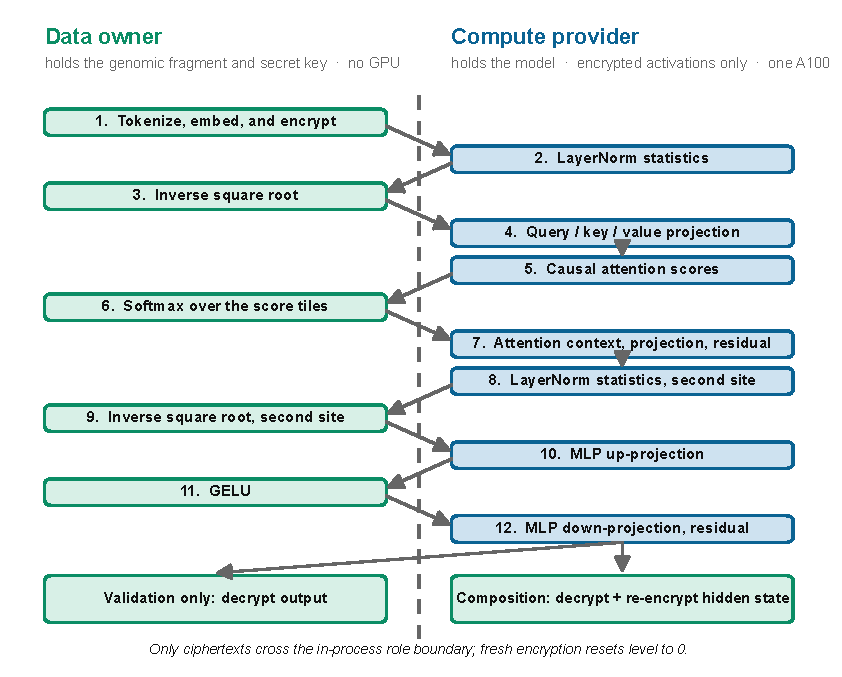
\includegraphics[width=\textwidth]{fig_architecture.pdf}
  \caption{Client-assisted block evaluation. The compute provider evaluates encrypted linear algebra
  and the data owner evaluates exact nonlinearities at declared boundaries. The provider has public
  weights, keys, and execution metadata, but receives no plaintext query-derived activation or secret key.}
  \label{fig:architecture}
\end{figure*}

\subsection{Client boundaries and normalization}
CKKS carries affine maps, reductions, residual additions, and attention products. The inverse
square root in LayerNorm, causal softmax, and GELU use declared client calls. At each call, the
data owner decrypts values derived from its query, evaluates the function in double precision, and
encrypts the result afresh under the same key. Algorithm~\ref{alg:boundary} gives this operation.

\begin{algorithm}[H]
\small
\caption{The client boundary. The data owner is the only party holding $\mathsf{sk}$, and every
value it decrypts derives from its own query.}
\label{alg:boundary}
\begin{algorithmic}[1]
\Function{ClientBoundary}{$c$, $f$}
  \State $v \gets \Call{Decode}{\Call{Decrypt}{\mathsf{sk},c}}$
  \State $v' \gets f(v)$ \Comment{evaluated exactly, in double precision}
  \State \Return $\Call{Encrypt}{\mathsf{pk},\Call{Encode}{v'}}$ \Comment{fresh ciphertext at
         level $0$}
\EndFunction
\end{algorithmic}
\end{algorithm}

Fresh encryption returns the activation to level~$0$. The configured depth of $13$ therefore bounds
the longest encrypted run between boundaries rather than the depth accumulated across all $12$
transformer blocks. The ciphertext lineage remains at the server between these calls.

For LayerNorm, the server computes the mean and centered variance under encryption and adds
$\varepsilon$ before sending the variance term to the client. Only the inverse square root is
evaluated there; the server then applies the returned factor and public scale, as specified in
Algorithm~\ref{alg:layernorm}. No bias is omitted as an approximation: the released checkpoint
contains no bias tensors.

\begin{algorithm}[H]
\small
\caption{LayerNorm. The server computes both statistics under encryption; only the inverse square
root crosses the boundary. The released checkpoint carries no bias term.}
\label{alg:layernorm}
\begin{algorithmic}[1]
\Function{LayerNorm}{$x$, $\gamma$}
  \State $\mu \gets \Call{ReduceSum}{x}\odot(1/D)$
  \State $z \gets x - \mu$
  \State $\sigma^2 \gets \Call{ReduceSum}{z \odot z}\odot(1/D) + \varepsilon$
  \State $r \gets \Call{ClientBoundary}{\sigma^2,\ t \mapsto t^{-1/2}}$
  \State \Return $(z \odot r) \odot \gamma$
\EndFunction
\end{algorithmic}
\end{algorithm}

\subsection{Packing and dense transforms}
The slot layout in Fig.~\ref{fig:packing} assigns $32{,}768$ slots as $4$ activation copies by
$1{,}024$ padded features by $8$ token lanes. Token lane is the innermost index: whole-lane
rotations move features without mixing tokens, and smaller rotations align token lanes. The
released width of $768$ occupies the active feature region; padding supports the power-of-two
transform and attention-score staging. Rows and columns outside the active width contribute zeros.

\begin{figure}[!t]\centering
  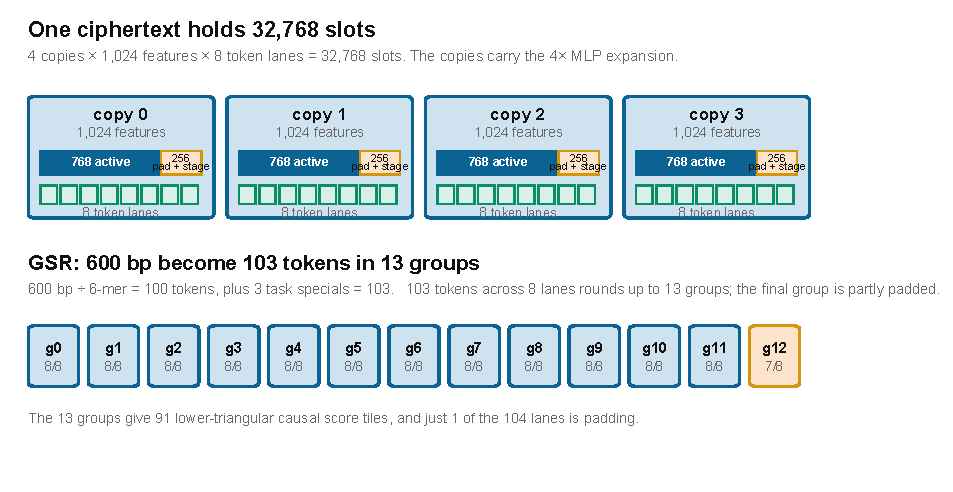
\includegraphics[width=\columnwidth]{fig_packing.pdf}
  \caption{Slot layout and grouping for the measured prompt. The final ciphertext group carries
  seven live tokens and one padded lane; the groups produce the lower-triangular causal score tiles.}
  \label{fig:packing}
\end{figure}

The four copies express the MLP expansion from width $768$ to $3{,}072$ as parallel chunks.
The $103$ tokens occupy $13$ ciphertext groups. A $32\times32$ baby-step giant-step decomposition
covers the $1{,}024$ padded features. Algorithm~\ref{alg:matmul} combines shared baby rotations
with encoded weight diagonals, cloning each plaintext for use at the receiving ciphertext's level.

\begin{algorithm}[H]
\small
\caption{Packed matrix product, baby-step giant-step over the packed diagonals.
$N_1 = N_2 = 32$ and $N_1N_2 = W = 1024$.}
\label{alg:matmul}
\begin{algorithmic}[1]
\Function{MatMul}{$\beta$, $M$}
  \State $d \gets \Call{EncodedDiagonals}{M,\ \mathrm{level}(\beta_0)}$
         \Comment{encoded once, cloned per use}
  \State $y \gets 0$
  \For{$j \gets 0$ \textbf{to} $N_2-1$}
    \State $u \gets \sum_{i<N_1} \beta_i \odot \Call{Clone}{d_{N_1 j + i}}$
    \State $y \gets y + (j = 0\ ?\ u : \Call{Rot}{u, B N_1 j})$
  \EndFor
  \State \Return $y$
\EndFunction
\end{algorithmic}
\end{algorithm}

Eight-token packing reduces the serial-equivalent dense-product count from $1{,}236$ to $156$,
a structural reduction of $7.92\times$. Rotations, masking, encoding, and client work remain, so
this operation-count ratio does not specify a latency speedup.

\subsection{Block evaluation}
\label{sec:algorithms}
Algorithm~\ref{alg:block} follows the released block through normalization, query/key/value
projection, causal attention, output projection, residuals, and the expanded MLP. The cached
diagonals are flushed after the last use of each weight set; this changes storage lifetime without
changing the arithmetic. Baby rotations are shared among transforms that consume the same input.

\begin{algorithm}[!t]
\small
\caption{Evaluating one transformer block. $G=13$ token groups; $\odot$ is homomorphic
multiplication; every operation outside a \textsc{Client} call runs on ciphertexts.}
\label{alg:block}
\begin{algorithmic}[1]
\Require encrypted activations $c_0,\dots,c_{G-1}$; public weights $W$
\Statex \textit{Stage 1: normalization and projection}
\For{$g \gets 0$ \textbf{to} $G-1$}
  \State $n \gets \Call{LayerNorm}{c_g,\ \gamma_1}$ \Comment{Algorithm~\ref{alg:layernorm}}
  \State $\beta \gets \Call{BabyRotations}{n}$ \Comment{$N_1-1$ rotations, shared}
  \State $Q_g \gets \Call{MatMul}{\beta,W_q}$; $K_g \gets \Call{MatMul}{\beta,W_k}$
  \State $V_g \gets \Call{MatMul}{\beta,W_v}$
\EndFor
\State \Call{FlushEncodedWeights}{} \Comment{bounds host memory to one stage}
\Statex \textit{Stage 2: causal attention scores}
\For{$k \gets 0$ \textbf{to} $G-1$}
  \State $\tilde{K} \gets \{\Call{LaneShift}{K_k,\delta}\}$ for each $\delta$ required by a
         later query group
  \For{$q \gets k$ \textbf{to} $G-1$}
    \State $S \gets 0$
    \For{$\delta \in \Call{ActiveShifts}{q,k}$}
      \State $P \gets Q_q \odot \tilde{K}_\delta$
      \For{$h \gets 0$ \textbf{to} $H-1$}
        \State $S \gets S + \Call{ReduceSum}{P \odot \mathrm{mask}_h} \odot
               \mathrm{isolate}(q,k,\delta,h)/\sqrt{d_h}$
      \EndFor
    \EndFor
    \State \Call{Client.TakeScoreTile}{$S,q,k$} \Comment{decrypt only}
  \EndFor
\EndFor
\State \Call{Client.Softmax}{} \Comment{stable softmax over complete causal rows}
\Statex \textit{Stage 3: attention context}
\For{$k \gets 0$ \textbf{to} $G-1$}
  \State $\tilde{V} \gets \{\Call{LaneShift}{V_k,\delta}\}$
  \For{$q \gets k$ \textbf{to} $G-1$; $\ \delta \in \Call{ActiveShifts}{q,k}$}
    \State $A \gets \Call{Client.EmitWeightTile}{q,k,\delta}$ \Comment{re-encrypt only}
    \State $C_q \gets C_q + A \odot \tilde{V}_\delta$
  \EndFor
\EndFor
\Statex \textit{Stages 4 and 5: projection, MLP, residuals}
\For{$g \gets 0$ \textbf{to} $G-1$}
  \State $R_g \gets c_g + \Call{MatMul}{\Call{BabyRotations}{C_g},W_{\text{proj}}}$
\EndFor
\State \Call{FlushEncodedWeights}{}
\For{$g \gets 0$ \textbf{to} $G-1$}
  \State $\beta \gets \Call{BabyRotations}{\Call{LayerNorm}{R_g,\gamma_2}}$
  \State $h \gets \sum_{c<4} \Call{MatMul}{\beta,W_{\text{fc}}^{c}} \odot \mathrm{copy}_c$
  \State $a \gets \Call{Client.GELU}{h}$
  \State $c'_g \gets R_g + \sum_{c<4}
         \Call{MatMul}{\Call{BabyRotations}{a \odot \mathrm{copy}_c},W_{\text{mlp}}^{c}}$
\EndFor
\State \Return $c'_0,\dots,c'_{G-1}$
\end{algorithmic}
\end{algorithm}

The protocol transcript is fixed by the circuit and sequence length. Each block makes $857$
physical client boundary crossings, including $91$ score-tile decryptions and $727$ weight-tile
encryptions. They carry $129{,}162$ logical nonlinear instances. Softmax accounts for $128{,}544$,
or $99.5\%$, of them, concentrating the boundary work in attention. The implementation asserts
the operation schedule, boundary counts, and remaining depth at run time and aborts on deviation.

\subsection{Causal attention}
Attention visits the $91$ lower-triangular pairs of the $13$ token groups. Shifts required by
later query groups are computed once per key group and reused. The client collects all encrypted
score tiles before stable softmax normalizes complete causal rows, then returns fresh encrypted
weight tiles for context aggregation. This normalization is a global synchronization point.

Both query--key scoring and weight--value aggregation multiply two activation-derived operands.
Of the block's $1{,}506$ ciphertext--ciphertext multiplications, LayerNorm contributes $26$
centered squares and $26$ products with returned inverse square roots. Attention contributes
$727$ query--key and $727$ weight--value products, or $97\%$ of the total.

\subsection{Depth, parameters, and composition}
The retained context has ring dimension $65{,}536$, $32{,}768$ usable slots, and a $128$-bit
classical security level. It uses $50$-bit scaling, a $60$-bit first modulus, $3$ hybrid
key-switching digits, and $80$ rotation keys. Depth $13$ is the smallest demonstrated passing
depth for these parameters and packing; the block finishes with $6$ levels remaining.

Between blocks, the data owner decrypts the full hidden state, restores its token-vector layout,
and encrypts fresh level-$0$ inputs under the same context and key lineage. The preliminary
two-block execution at two tokens reached relative error $8.48\times10^{-11}$ without GPU-memory
growth in the second block. Section~\ref{sec:results} reports the complete task-length composition.

\subsection{Non-interactive comparison}
The non-interactive design replaces every nonlinearity with a polynomial approximation and
retains a single ciphertext lineage without intermediate decryption. It completes one
released-weight block. When configured for composition, however, its context and evaluation keys
exceed the tested $80$~GB GPU-memory envelope before useful composition arithmetic begins.

Repeated polynomial evaluation requires a deeper modulus budget and a bootstrapping schedule
whose associated material must remain resident. This memory limit applies to the tested library,
parameters, packing, and hardware. The client-assisted design shortens encrypted segments by
evaluating the exact functions at the client and refreshing through fresh encryption.

% ---------------------------------------------------------------------------
% 6 Optimization -- the systems core of the paper
% Source: evidence/optimizations.yaml (authoritative), docs/hybrid/t123_walkthrough.md §7, §9
% Discipline: the operation schedule is identical at every step. Say so up front; it is what
% makes the speedup attributable to systems work rather than to a cheaper circuit.
%
% Tone: this section is the good news and should read that way. Abandoned attempts appear only
% where they explain a retained design choice (the clone, and the sequential client boundary),
% one or two sentences each, in the subsection they explain. No catalogue of failures.
% Only timing artifacts that satisfy the manuscript evidence rule may appear in the paper.
% ---------------------------------------------------------------------------

\section{Host-side systems work at fixed circuit}
\label{sec:optimization}

Encoding each distinct weight diagonal once removes redundant host work but creates a memory
lifetime problem. An implementation that retained every encoded template was terminated by the
operating system at $61{,}863$~MiB resident, when the MLP began building templates on top of those
cached by earlier stages. Bounding the cache to one live stage makes reuse executable within the
tested host-memory envelope. Peak host memory is then determined by the largest stage, not by every
encoded weight in the block. The remaining changes govern when host data are prepared, how long
they remain resident, and where CPU work executes.

Every change in this section holds the encrypted circuit fixed: the retained implementation executes
the same checked operation schedule before and after each change, with packing, multiplicative
depth, boundary order, and the frozen plaintext reference unchanged, and the run-time checks of
Section~\ref{sec:protocol} abort on any deviation. No retained change removes a dense transform,
reduces the number of attention tiles, moves linear algebra to the client, or relaxes the acceptance
criterion. The section therefore reports verified changes in executed work and memory but no
elapsed-time comparison, because no dedicated-node measurement of the pre-optimization configuration
exists.

\subsection{Host-side encoding redundancy}
The baseline rebuilt and encoded every packed diagonal for every dense product. Its $156$ products
each required $1{,}024$ diagonal plaintexts, producing $159{,}744$ encoding operations per block,
and about $90\%$ of that work was byte-identical: the block has $12$ weight matrices, each used
across all $13$ token groups. The GPU could not begin a multiplication until the host had prepared
its plaintexts.

In the baby-step giant-step transform, a plaintext diagonal is not merely a view of the original
matrix: it must be packed, scaled, and encoded for the ciphertext level at which multiplication will
occur. Repeating that conversion for every token group made a model-invariant representation step
dominate the call path. The optimization target is therefore the lifetime and placement of plaintext
preparation, while the encrypted products and accumulations remain fixed.

\subsection{Encode once, clone per use}
The retained cache encodes each distinct weight diagonal into a pristine host template. A
multiplication receives a lightweight clone that shares the encoded host data by reference while
carrying fresh device state; the clone is loaded and evicted for that operation. This removes
$90\%$ of the $159{,}744$ encoding operations without keeping a plaintext object resident on the
GPU between multiplications.

Cloning is required by the evaluated backend's object semantics. Its plaintext-load path returns
early when an object is already marked as loaded, so directly reusing a template across
multiplicative levels can pair a new ciphertext level with stale residue-number-system limbs.
Fresh device state on each clone forces a load at the level required by the current operation. An
isolated GPU micro-test checked clone-versus-fresh-encode equality, cross-level reuse, stable device
memory under repeated multiplication, and equality between parallel and serial encoding before the
cache was applied to the complete block.

Templates are indexed by both weight matrix and multiplicative level, which preserves the backend's
level contract while still sharing work among token groups that reach the same matrix at the same
level. The cache therefore stores reusable encoded data, not a ciphertext or a mutable GPU object,
and leaves homomorphic multiplication itself unchanged.

\subsection{Bounding host memory}
Removing repeated encoding exchanges computation for host memory. An early cache retained
templates from every completed stage, and the process did not survive the MLP. Two exact changes
bound the cache. First, a template is encoded directly at its multiplicative level of use, so it
carries only the limbs needed by the receiving ciphertext; this changes no arithmetic, because the
backend would otherwise drop a level-$0$ plaintext to the same level before multiplication. Second,
the implementation flushes the cache after query/key/value projection and after the attention
projection, which are the final use sites for their respective weight sets: no weight matrix recurs
across either boundary, so retaining those templates cannot produce another hit.

The lifetime policy follows the block topology. Within a stage, the group-major loop revisits its
weights as it advances through token groups, so early eviction would discard real reuse; across
stages, the next operation consumes a different set of weights, so eviction there releases memory
without creating a later re-encoding.

The target-process resident-set trace follows this policy, as
Figure~\ref{fig:systems}(d) shows. Query/key/value projection reaches
$25{,}530$~MiB. Attention begins after a flush and uses $12{,}434$~MiB. The MLP holds eight
matrices and reaches the block peak of $48{,}610$~MiB. The largest live stage, rather than every
encoded weight in the block, determines peak host memory.

\subsection{Placement and parallelism}
Plaintext preparation also depends on where host work runs. The retained implementation binds
threads to physical cores and uses NUMA-local allocation so encoding threads stay close to the
memory they allocate and to buffers staged for the GPU; decryption, exact nonlinear evaluation, and
re-encryption use the same host resources. Template construction is then batched across the
available $32$ cores with dynamic scheduling, since each diagonal can be encoded independently
without changing the order or result of encrypted multiplications; parallel and serial construction
were checked for equal outputs before the parallel path was retained. Affinity controls placement
and batching exposes independent diagonals to the cores, so together they make plaintext preparation
a core-local parallel batch under the same cryptographic parameters. Their elapsed-time effect
awaits a sourced paired measurement.

\begin{table*}[!tb]\centering\small
\caption{Host-side changes at fixed circuit. Every row leaves the operation schedule, packing,
multiplicative depth, and frozen plaintext reference unchanged. Effects are verified changes in
executed work or in memory; the table carries no elapsed-time column, because no dedicated-node
measurement of the pre-optimization configuration exists.}
\label{tab:optimization}
\begin{tabularx}{\linewidth}{Y l l}
\toprule
Change & Verified effect & Status \\
\midrule
Re-encode every plaintext per multiplication & $159{,}744$ encodings & baseline \\
Thread affinity, NUMA-local allocation & host placement changed & retained \\
Encode once, clone per use & removes $90\%$ of encodings & retained \\
Parallel batched encoding & equal to serial encoding & retained \\
Encode at use level, flush between stages & peak $48{,}610$~MiB RSS & enabling \\
\midrule
\textbf{Net} & \textbf{checked operation schedule unchanged} & \\
\bottomrule
\end{tabularx}
\end{table*}

% No waterfall figure: it needs two supported timing endpoints, and the pre-optimization
% baseline has no committed dedicated-node measurement. The generator is retained in
% scripts/figures.py but is not registered in FIGURES.

\subsection{Remaining optimization targets}
Mask plaintexts are still encoded afresh at approximately $17{,}400$ uses per block. Head masks,
score-isolation masks, lane masks, and copy-activity masks all have fixed values under the declared
layout, so host templates could remove the same class of repeated work already eliminated for
weight diagonals. This target remains unimplemented.

A second opportunity lies in the four packed activation copies. They currently carry duplicates
through a dense transform. An analyzed layout would apply distinct transforms to those copies,
placing query, key, and value projections together and likewise combining the MLP expansion
chunks. At fixed model arithmetic, the projected schedule reduces dense products from $156$ to
approximately $52$ and dense ciphertext--plaintext multiplications from $159{,}744$ to
approximately $53{,}248$; the total ciphertext--plaintext count falls by roughly $60\%$ before mask
and copy-repair overhead. This is a derived projection for an unimplemented layout, and it requires
an exact reconstruction proof before implementation.

Client work has a separate opportunity. Attention dominates the boundary schedule
(Section~\ref{sec:protocol}), and each attention tile's cryptographic work is independent.
Concurrent client boundaries were unsafe under the evaluated shared crypto context, so the retained
implementation executes them sequentially. A thread-safe context would expose this independent work
to concurrency.

% ---------------------------------------------------------------------------
% 7 Results
% Every number here comes from evidence/measurements.yaml, telemetry.yaml, or scaling.yaml.
% The complete-model timings come from the dedicated-node run of 2026-08-12 (n = 1).
% Per-block timings sourced only to the shared-partition walkthrough remain withheld.
% ---------------------------------------------------------------------------

\section{Results}
\label{sec:results}

The client-assisted circuit defined in Section~\ref{sec:protocol} is evaluated along four axes:
numerical agreement, the executed operation schedule, memory, and the cost of a complete encrypted
inference. The complete model has been executed once on an uncontended node, and that single
execution is the source of every timing reported here. Per-block timings from earlier
shared-partition runs are not reported, because host contention cannot be separated from the
measurement after the fact.

\subsection{Correctness}

Correctness rests on the two-stage chain described in Section~\ref{sec:baseline}. Before encrypted
evaluation, the independent NumPy reference is asserted against the upstream PyTorch computation at
a tolerance of $2\times10^{-5}$, separately for all $12$ transformer blocks and the classifier
head; export aborts on a divergence. The encrypted circuit is then compared with that validated
reference. This ordering prevents an unchecked reimplementation from serving as the sole judge of
its encrypted counterpart.

For one block at the $103$-token task prompt, the decrypted output has relative infinity-norm error
$4.64\times10^{-9}$ against an acceptance tolerance of $4\times10^{-2}$ fixed before the run,
leaving seven orders of magnitude of headroom. The worst token-relative error is
$4.7\times10^{-9}$, and the largest absolute deviation is $7.44\times10^{-8}$. These values
establish numerical agreement for the encrypted block with the released weights and exact client
nonlinearities.

The complete model is held to the same unchanged tolerance. Evaluating all $12$ released blocks
and the released task head at the $103$-token task prompt yields a decrypted classification margin
that differs from the plaintext oracle margin by $8.56\times10^{-9}$ in relative terms and
$1.05\times10^{-7}$ in absolute terms, and the decrypted class label matches the frozen reference
label.

Error does accumulate with depth, and the size of that accumulation is the useful result. The
hidden-state relative infinity norm is $4.09\times10^{-9}$ after the first block and
$2.07\times10^{-8}$ after the twelfth, while the largest absolute deviation grows from
$6.56\times10^{-8}$ to $7.97\times10^{-6}$, roughly two orders of magnitude across the model.
Growth of that rate leaves the twelfth-block activation six orders of magnitude inside the
acceptance tolerance, and leaves the margin the classifier actually acts on inside it by nine. The
claim is therefore not that approximation error fails to accumulate, but that it accumulates far
too slowly over this depth to change the decision.

\subsection{Executed work}

\begin{table}[t]\centering\small
\caption{Checked operation schedule for the evaluated transformer block.}
\label{tab:cost}
\begin{tabularx}{\textwidth}{Y r l}
\toprule
Operation & Count & Executor \\
\midrule
Dense products & 156 & compute provider \\
Ciphertext--plaintext multiplications & 177{,}734 & compute provider \\
Ciphertext--ciphertext multiplications & 1{,}506 & compute provider \\
Rotations & 8{,}173 & compute provider \\
Slot reductions & 8{,}776 & compute provider \\
Physical client boundary crossings & 857 & data owner \\
Logical nonlinear values & 129{,}162 & data owner \\
\bottomrule
\end{tabularx}
\end{table}

The implementation asserts every count in Table~\ref{tab:cost}, the boundary sequence, and the
remaining multiplicative depth before the MLP. Any deviation aborts the run. This turns the
operation schedule into evidence that the optimized implementation executes the same circuit, not
an assurance inferred from a passing output.

Packing separates physical interaction from nonlinear model work. The $857$ physical client
boundary crossings carry $129{,}162$ logical values. Softmax accounts for $128{,}544$ of those
values, or $99.5\%$; LayerNorm and GELU together account for the remainder. Boundary optimization
is therefore principally an attention problem, even though the protocol contains three
nonlinearity classes.

The dense schedule also records the benefit of token packing. Eight-token packing reduces the
serial-equivalent dense-product count from $1{,}236$ to $156$, a $7.92\times$ reduction in
operations. Rotations, masking, client work, and host preparation remain in the packed circuit, so
the factor describes operation count rather than latency.

\subsection{Memory}

The evaluating process peaks at $9839$~MiB of GPU memory, within the $40$~GB device used for the
experiment. This is the evaluating process footprint rather than device-wide occupancy.

Host memory follows the lifetime of encoded plaintext templates. Query/key/value projection reaches
$25{,}530$~MiB of target-process resident memory. A cache flush precedes attention, whose recorded
resident memory is $12{,}434$~MiB. The MLP holds the largest live weight set and reaches the block
peak of $48{,}610$~MiB. These stage transitions match the explicit flush points in
Section~\ref{sec:optimization}; encoded weights do not accumulate across the entire block.

The two memory results have different mechanisms. The non-interactive composition configuration
exceeded its tested $80$~GB GPU envelope while loading the deep context and evaluation keys.
Client re-encryption shortens the encrypted segments and resets their depth budget, moving that
accelerator-memory barrier. Stage-bounded caching prevents the resulting host-side plaintext
templates from becoming an unbounded second barrier.

\begin{figure}[tb]\centering
  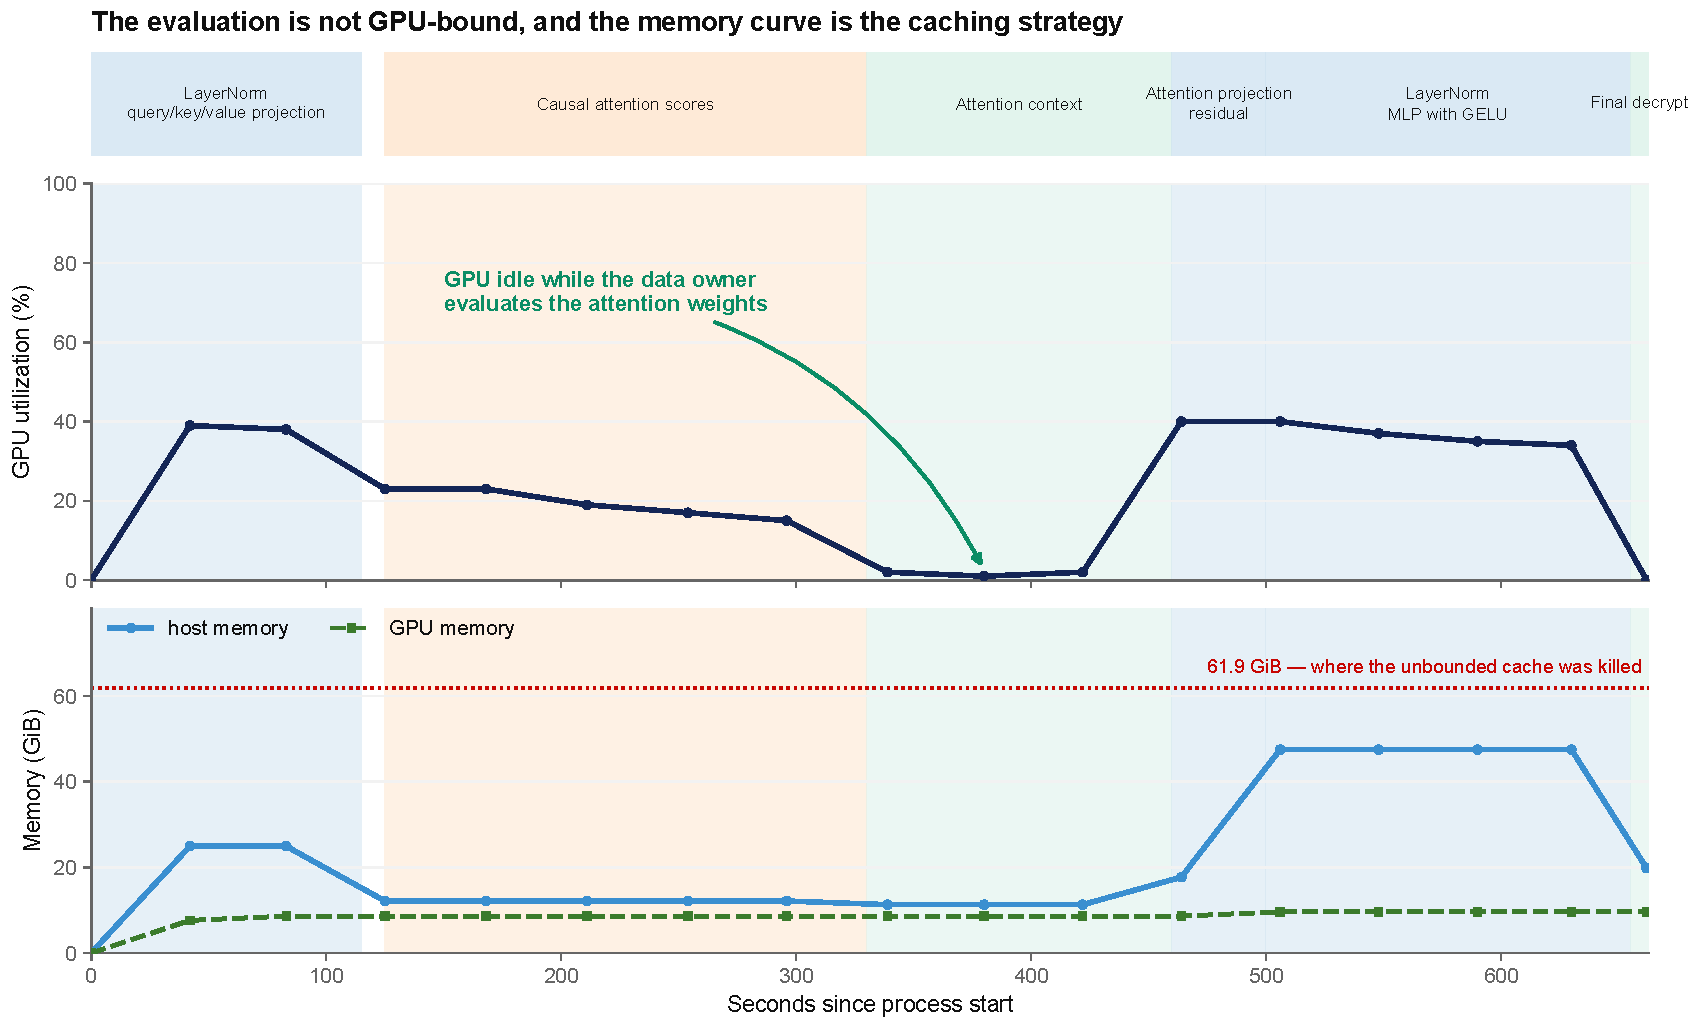
\includegraphics[width=\textwidth]{fig_timeline.pdf}
  \caption{Resource trace of the complete encrypted inference. GPU utilization never exceeds $51\%$, so the evaluation is not accelerator-bound even at whole-model scale. Host memory oscillates once per block, following the stage flushes of Section~\ref{sec:optimization}, rather than accumulating across the twelve blocks; GPU memory reaches its peak during the first block and does not grow with block index. The twelve cycles are the twelve blocks.}
  \label{fig:timeline}
\end{figure}

The complete model confirms that both bounds hold at full depth. GPU memory rises during context
and key loading, reaches $9839$~MiB after roughly $400$~s, and then holds that value exactly for
the remainder of the run: the same footprint the single block reaches, with no growth in block
index; host resident memory peaks at $50{,}930$~MiB, consistent with the same MLP-stage maximum
recurring once per block rather than accumulating. The memory barrier that stopped the
non-interactive configuration evaluated here is therefore not deferred by client assistance but
removed: twelve blocks cost what one block costs.

\subsection{Composition and evaluation boundary}

\begin{table}[t]\centering\small
\caption{Encrypted evaluation completed at each reported scope. Hidden-state error is a
relative infinity norm over the activation; margin error is the scalar the classifier acts on.
The two are different quantities and are kept in separate columns.}
\label{tab:scope}
\begin{tabularx}{\textwidth}{Y l l l}
\toprule
Scope & Status & Hidden-state error & Margin error \\
\midrule
One block, 2 tokens & measured & --- & --- \\
Two consecutive blocks, 2 tokens, client refresh & measured & $8.48\times10^{-11}$ & --- \\
One block, 103 tokens (task length) & measured & $4.64\times10^{-9}$ & --- \\
Twelve blocks and task head, 103 tokens & measured & $2.07\times10^{-8}$ & $8.56\times10^{-9}$ \\
Encrypted token-index lookup & out of scope & --- & --- \\
\bottomrule
\end{tabularx}
\end{table}

Two consecutive released blocks compose at reduced sequence length through a full-hidden-state
client refresh, reaching $8.48\times10^{-11}$ relative error after the second block. GPU memory
peaks in the first block and does not increase in the second. This experiment checks the mechanism
used for deeper composition: a fresh encryption starts the next block at level~$0$ without
carrying forward the preceding block's multiplicative depth or GPU-resident temporaries.

The complete model exercises that mechanism eleven more times. All $12$ blocks and the task head
run in one key lineage, separated by $11$ full-hidden-state refreshes between consecutive blocks
and one further refresh of the final token into the head. Multiplicative depth stays at $13$
throughout, the same budget the single block requires, and the run performs no homomorphic
bootstrap at any point. Depth is thus a property of the longest segment between two client
boundaries rather than of network depth, which is what makes a twelve-block encrypted lineage
expressible at all under these parameters.

\subsection{Cost of a complete encrypted inference}

\begin{figure}[tb]\centering
  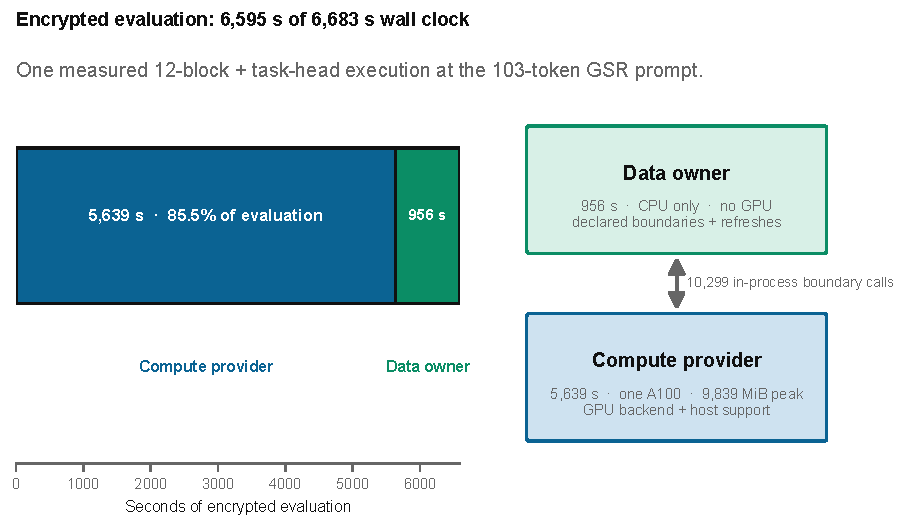
\includegraphics[width=\textwidth]{fig_cost_split.pdf}
  \caption{How one complete encrypted inference divides between the two parties. The compute provider performs the encrypted linear algebra on one A100; the data owner evaluates the nonlinearities on CPU with no GPU. Server and client shares sum exactly to encrypted evaluation. Single execution on an uncontended node.}
  \label{fig:costsplit}
\end{figure}

\begin{table}[t]\centering\small
\caption{One complete encrypted inference: twelve blocks and the released task head at the
$103$-token task prompt, on one A100 GPU node using 32 CPU threads. Single execution on an
uncontended node; these are one sample's values, not averages over repetitions. Shares are rounded
independently and need not sum to $100\%$.}
\label{tab:fullcost}
\begin{tabularx}{\textwidth}{Y r r}
\toprule
Phase & Seconds & Share of wall \\
\midrule
Load released weights and verified reference & 23.494 & 0.4\% \\
Crypto context, key generation, GPU key upload & 3.945 & 0.1\% \\
Encrypt the embedded input & 1.265 & 0.0\% \\
\textbf{Encrypted evaluation} & \textbf{6594.748} & \textbf{98.7\%} \\
\quad server linear algebra (GPU) & 5638.561 & 84.4\% \\
\quad client boundaries (CPU, exact) & 956.187 & 14.3\% \\
Final decrypt & 0.044 & 0.0\% \\
Uninstrumented remainder & 59.504 & 0.9\% \\
\midrule
\textbf{Wall clock} & \textbf{6683} & \\
\bottomrule
\end{tabularx}
\end{table}

A complete encrypted inference takes $6683$~s of wall clock, or $1.86$~hours. Encrypted evaluation
accounts for $6594.748$~s of that, and setup is negligible at this scale: context construction and
key generation together take under four seconds, and the single final decryption takes $0.044$~s.
The instrumented phases are a decomposition rather than a partition, leaving $59.504$~s, or $0.9\%$
of wall clock, outside them; Table~\ref{tab:fullcost} shows that remainder rather than distributing
it silently.

Within encrypted evaluation the split between the two parties is exact: server linear algebra uses
$5638.561$~s and the data owner's boundary work uses $956.187$~s, and the two sum to the evaluation
total without residue. The compute provider therefore carries $85.5\%$ of the encrypted work and
the data owner $14.5\%$, with the data owner's share running on CPU alone. Across $10{,}299$
physical boundary crossings the mean crossing costs $0.093$~s, and those crossings carry
$1{,}551{,}081$ individual nonlinear values, so the interaction count understates the nonlinear work
by more than two orders of magnitude.

The twelve blocks account for $6565.993$~s and the encrypted task head for $9.046$~s, so the head
is not a meaningful part of the cost. The twelve refreshes together cost $19.710$~s, which places
the price of the composition mechanism at roughly $0.3\%$ of encrypted evaluation. Dividing block
evaluation by twelve gives $547.166$~s per block. The twelve individual block times span
$533.869$~s to $558.943$~s, a spread of $4.7\%$ across architecturally identical blocks on one
node. That bounds within-run scheduling jitter; it is not run-to-run variance, which a single
execution cannot report.

\subsection{Sequence-length structure}

\begin{figure}[tb]\centering
  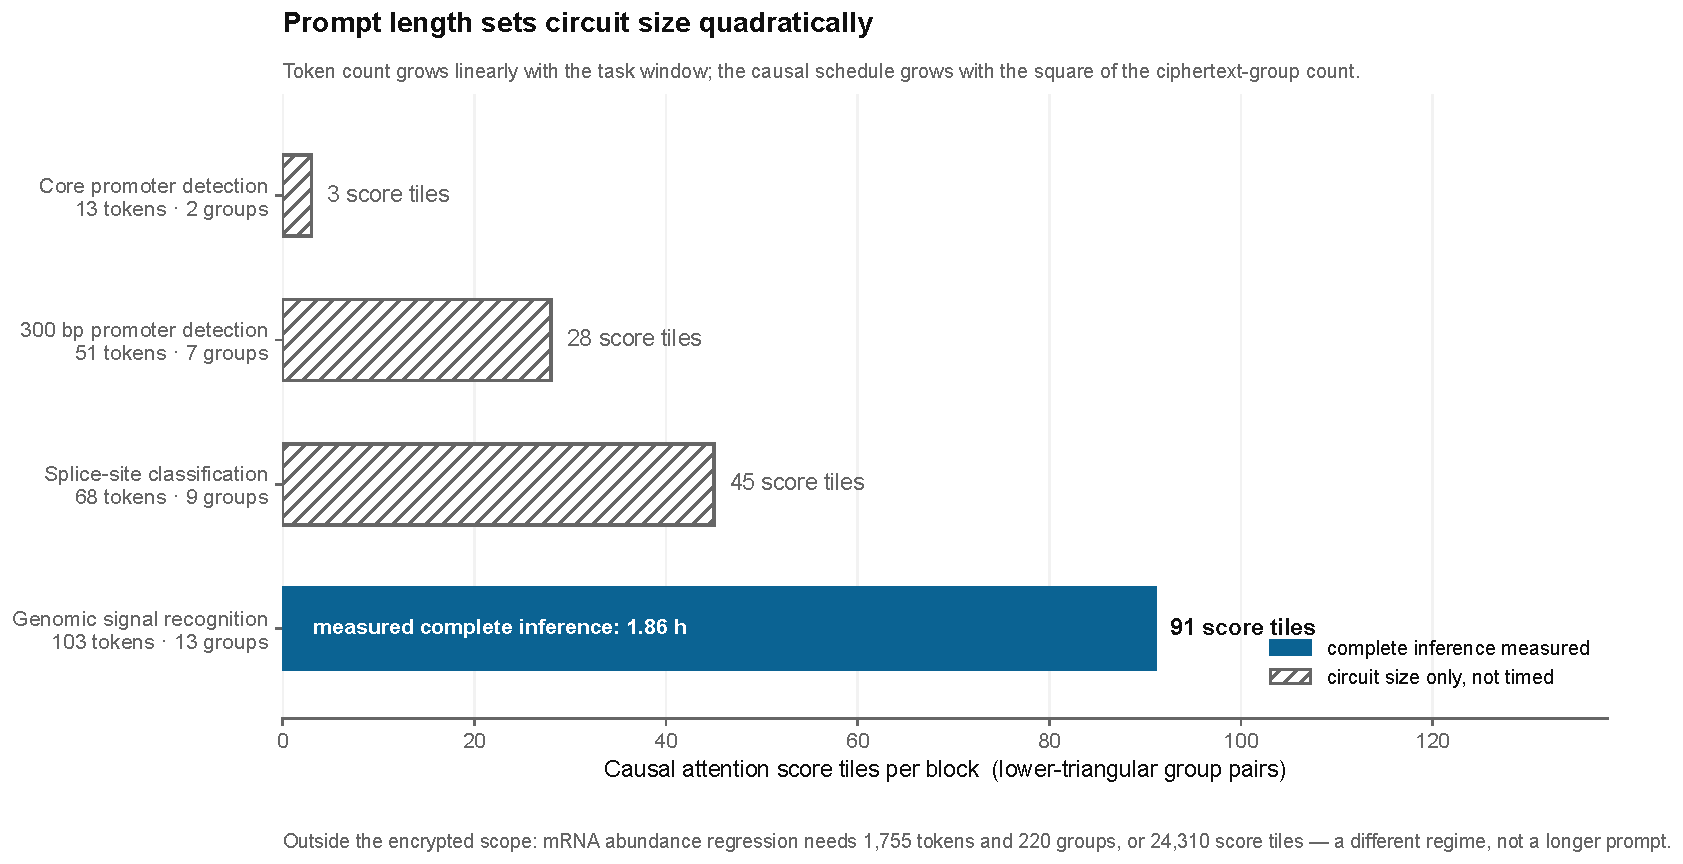
\includegraphics[width=\textwidth]{fig_scaling.pdf}
  \caption{Circuit size across the encrypted-scope tasks. The bars show causal attention score tiles per block, which follow from the ciphertext-group count and not from any timing model; only genomic signal recognition has a measured complete encrypted inference. Token counts follow from each task's window under 6-mer tokenization.}
  \label{fig:scaling}
\end{figure}

Sequence length follows from each task format. Genomic-signal recognition uses $600$ base pairs,
which become $100$ sequence tokens under $6$-mer tokenization; three task-format tokens produce the
$103$-token encrypted anchor. Eight-token packing maps that prompt to $13$ ciphertext groups. The
shorter promoter and splice-site prompts use fewer groups under the same layout, yielding smaller
causal schedules.

The abundance-regression task lies outside the encrypted scope. Its $10{,}500$ base pairs produce
$1{,}755$ tokens and $220$ ciphertext groups under the same tokenization rule. The causal attention
schedule grows quadratically in the number of groups, placing this task in a different circuit-size
regime from the classification prompts.

\subsection{Feasibility}
\label{sec:verdict-feasibility}

Complete encrypted inference for DNAGPT is feasible under the stated protocol. All $12$ released
blocks and the released task head evaluate at the task's own prompt length in a single key lineage,
and the decrypted prediction reproduces the frozen plaintext label with $8.56\times10^{-9}$
relative margin error against a tolerance fixed before the run. The claim is no longer an argument
from a block plus a composition mechanism; the complete computation has been run and accepted.

Three properties make that outcome more than a single passing execution. Multiplicative depth stays
at $13$ across the whole model, so depth is bounded by the longest segment between client
boundaries and not by network depth. GPU memory holds at $9839$~MiB once loading completes, rather than
growing with block index, so composition does not accumulate accelerator state. And no
homomorphic bootstrap is performed anywhere, which is what removes the deep-context and
evaluation-key residency that stopped the non-interactive configuration evaluated in
Section~\ref{sec:protocol}. Correctness, depth, and accelerator memory are therefore all resolved
for a complete model at task length. Whether they would have obstructed a different
non-interactive implementation is not settled by this study, and Section~\ref{sec:related} reports
prior systems that do not encounter the same envelope.

What remains outside this verdict is the encrypted token-index lookup, which the protocol does not
attempt, and the transport layer, which is evaluated in one process rather than across a network.
Section~\ref{sec:limitations} states both.

\subsection{Practicality, judged separately}
\label{sec:verdict-practicality}

Feasibility does not make the system practical, and the measured cost says so plainly. One
encrypted classification of one $600$-base-pair sequence occupied an A100 node for $1.86$~hours,
against a plaintext forward pass of the same released model that completes in well under a second
on commodity hardware. That rules out interactive per-query use outright. It does not rule out batch or offline analysis of
a sample set where disclosing the sequence is unacceptable and the alternative is not analysing it
at all, since in that setting hours per sequence is a cost rather than a barrier.

The comparison that decides the verdict, however, is not against plaintext inference but against
other encrypted systems, and it does not favour this design. THOR reports $602$~s for a
non-interactive encrypted forward pass of a $12$-layer, $768$-wide encoder at $128$ tokens on a
single A100, at the ring degree, multiplicative depth, and security level used here, with no client
participation at any point~\cite{thor}; MOAI reports a further reduction against
that~\cite{moai2025}. The $6683$~s measured here is roughly an order of magnitude above it at a
shorter prompt. The practicality verdict is therefore negative in two distinct senses: too slow for
interactive use in absolute terms, and behind the non-interactive state of the art in relative
terms. Section~\ref{sec:related} sets out what the design offers in exchange, which is exactness,
freedom from bootstrapping, and an output verifiable against a plaintext reference, rather than
speed.

Two qualifications bound how far our own number should be carried, and both of them widen rather
than narrow the gap above. It is a single execution, so it supports a statement about the cost of
this inference and not a distribution, a mean, or a service rate; repeated runs would be needed
before quoting a latency target. And it is measured in one process, so it excludes the serialization
and network transport that a deployed service would add to every one of the $10{,}299$ boundary
crossings, whereas a fully non-interactive system incurs no such transport at all. The comparison is
therefore generous to the design evaluated here.

The measurement also indicates that this cost is not a floor imposed by cryptography. GPU
utilization holds a median of $32\%$ and a maximum of $51\%$ across the complete run, so the
evaluation is not limited by accelerator throughput even at whole-model scale; the cost sits in
host-side encoding and in the sequential client boundary, which
Section~\ref{sec:optimization} identifies as addressable. Feasibility and practicality thus resolve
differently and for different reasons: the encrypted path is correct and complete, while its
present latency confines it to batch and offline use.

% ---------------------------------------------------------------------------
% 8 Limitations
% Source: context/05_claims_and_qualifiers.md, docs/hybrid/t123_walkthrough.md §11
% Discipline: this is where caveats LIVE. Do not scatter them through earlier sections.
% ---------------------------------------------------------------------------

\section{Limitations}
\label{sec:limitations}

The measured unit is one complete released-weight transformer block at the task's full
$103$-token prompt length, with encrypted server-side linear algebra and client-evaluated
nonlinearities. It does not include the remaining transformer blocks, the released task head, or
token-index lookup. The $12$-block driver with the task head is built but has not run at this prompt
length. The study reports no encrypted task accuracy or encrypted final prediction.

Client and server are roles inside one program on one node. Boundary calls perform the
cryptographic operations directly, without ciphertext serialization, network transport, or a key
custody service. A physical client boundary crossing is therefore not a network message. A
deployment experiment must measure serialized payload volume, dependency phases, bandwidth
sensitivity, transport latency, and production key handling rather than infer them from the
in-process counter.

Encryption begins at embedded numeric vectors. Tokenization, token-index lookup in the embedding
table, and construction of the initial embedding occur before the encrypted boundary. Private
lookup is therefore an unresolved part of a complete genomic inference service; none of the block
results closes it.

Model confidentiality remains operational rather than cryptographic. Because the data owner sees
full activations at every nonlinearity, the transcript divides the network into shallow segments
with known nonlinearities. Weight recovery becomes inexpensive per-segment regression instead of a
global inversion problem. Server-side weight placement can discourage casual copying but cannot
protect the model from a determined client; the deployment keeps the model on the server because
the server operates it.

The exposure is structural. MLP boundaries reveal inputs and corresponding pre- or post-activation
values for a shallow linear segment, while attention boundaries reveal score and weight relations.
Changing query policy may limit casual collection of such pairs, but it does not turn the transcript
into a cryptographic model-protection mechanism.

CKKS decryption is approximate. The client never returns a decoded value to the server, only a
freshly encrypted result, but the server selects the ciphertext supplied to each declared
boundary. The semi-honest threat model rules out adversarially chosen deviations from that
schedule. The current re-encryption path applies no noise flooding. The measured
$4.64\times10^{-9}$ error leaves seven orders of magnitude inside the $4\times10^{-2}$ acceptance
tolerance, but numerical headroom alone does not establish a secure flooding parameter. Selecting
and validating that budget remains future work.

The adversary exclusions are defined in Section~\ref{sec:threat-model}. The results do not extend
beyond that threat model.

% ---------------------------------------------------------------------------
% 10 Conclusion and closing statements
% ---------------------------------------------------------------------------

\section{Conclusion}

This study gives a split answer to the question of encrypted DNAGPT inference. Client-assisted CKKS
executes all twelve released blocks and the task head at the $103$-token prompt from encrypted
embedded vectors. For the one input evaluated, the decrypted label matches the frozen reference and
its margin has $8.56\times10^{-9}$ relative error against the $4\times10^{-2}$ predeclared tolerance.
Graph feasibility is established for the complete released computation; numerical generality
beyond this input is not. Client refresh bounds depth by the longest encrypted segment,
device-wide GPU memory used stays at $9839$~MiB across the blocks, and no homomorphic bootstrap is
required. A stage-bounded plaintext cache separately prevents host-memory accumulation.

Cost is the constraint that remains. One encrypted classification of one $600$-base-pair sequence
was measured at $1.86$~hours on an A100 GPU node, which forecloses interactive use in the evaluated
form. It is a single-process, single-input, single-execution result rather than a service-rate or
network measurement, and sampled GPU utilization peaking at $51\%$ indicates unclaimed headroom
without identifying its cause. The two verdicts are therefore separate, and both are informative:
complete-model feasibility is established for the executed case, practicality is not, and the
obstacle between them is engineering throughput on the provider's encrypted path rather than
correctness, multiplicative depth, or accelerator memory.

\subsection*{Future work}

Further empirical work would require additional prompts, repeated timings, and a paired
pre-optimization measurement; none is inferred from the present run. Systems work should extend the
encode-once strategy from weight diagonals to mask plaintexts. Distinct transforms across the
packed activation copies are the larger circuit opportunity. Before mask and copy-repair overhead,
the derived schedule for that layout projects a reduction of roughly $60\%$ in the block's total
ciphertext--plaintext count. A thread-safe cryptographic context would permit concurrent independent
client boundaries. Protocol closure also requires a noise-flooding budget for re-encryption. A
deployment study must add serialized network transport and private token-index lookup before
measuring the complete service.

\section*{Ethics statement}

This study involved no human participants, specimens, or private clinical records. It used public
reference datasets with recorded provenance. The work makes no clinical-performance claim and
does not present the prototype as a deployable privacy guarantee beyond its stated threat model.

\section*{Data availability statement}

All evaluation datasets are public. Their original sources, versions, preprocessing, and any
recovery route used are recorded in the repository's data-provenance document. Sequence data,
model weights, and cryptographic keys are not redistributed.

\section*{Code availability statement}

The evaluation harnesses, encrypted-evaluation implementation, environment definitions, and the
evidence record for the paper are maintained at
\url{https://github.com/Georgakopoulos-Soares-lab/private_genomic_dnagpt}. No repository-level
reuse license has yet been assigned.

% ---------------------------------------------------------------------------
% Submission declarations. References follow this file and therefore remain the
% final numbered material in the manuscript.
% ---------------------------------------------------------------------------

\section*{Ethics Statement}

This study involved no human participants, specimens, or private clinical records. It used public
reference datasets with recorded provenance. The work makes no clinical-performance claim and
does not present the prototype as a deployable privacy guarantee beyond its stated threat model.

\section*{Data Availability Statement}

All evaluation datasets are public. Their original sources, versions, preprocessing, and any
recovery route used are recorded in the repository's data-provenance document. Sequence data,
model weights, and cryptographic keys are not redistributed.

\section*{Code Availability Statement}

The evaluation harnesses, encrypted-evaluation implementation, environment definitions, and the
evidence record for the paper are maintained at
\url{https://github.com/Georgakopoulos-Soares-lab/private_genomic_dnagpt}. No repository-level
reuse license has yet been assigned.

% TODO(authors): insert an IEEE-style \section*{Acknowledgment} only after the
% funding and compute-allocation wording is supplied and approved by all authors.


\FloatBarrier
\bibliography{refs}

\end{document}
